In this chapter I report the initial results from the first test. After that I propose changes to this first test, and report the results from this final test.


\section{Evaluation Method}
\label{sec:eval_meth}
In order to find the best model on the dataset, I have created multiple models, each with different hyperparameters and combinations of features as input. I then tried to create a model for each possible combination of hyperparameters on each feature combination. Each model was created using the Keras \cite{Chollet2015keras} machine learning framework originally build for Python. This framework is build on top of the popular, well-known machine learning API \textit{Tensorflow 2.0} \cite{Tensorflow2015whitepaper}.

\subsection{The Hyperparameters}
\begin{table}[b]
    \centering
    \begin{tabular}{|l|l|}
    \hline
    \textbf{Hyperparameter} & \textbf{Values}                    \\ \hline\hline
    Neurons                 & 128, 256, 512                      \\ \hline
    Activation function     & \textit{ReLu, Elu}                 \\ \hline 
    Pooling                 & \textit{no\_pooling, max, average} \\ \hline
    Optimizer               & \textit{RMSprop, Adam}             \\ \hline
    Dropout                 & 10\%, 20\%, 30\%, 40\%, 50\%       \\ \hline
    Epochs                  & 1, 10, 50, 100                     \\ \hline
    Batch size              & 1, 5, 10, 50, 100                  \\ \hline
    \end{tabular}
    \caption{Initial hyperparameters and their initial range of values.}
    \label{tab:init_params}
\end{table}
For each generally important parameter for a neural network I've created a hyperparameter. I will explain each hyperparameter below. A list of all hyperparameters and their values can be found in \autoref{tab:init_params}.

\subsubsection{Neuron Count}
The first hyperparameter is the amount of neurons that make up the first layer, the first convolutional layer for the CNN models and the first or only B-LSTM layer of the LSTM models. I've chosen 128, 256 and 512 as possible neuron counts. 

\subsubsection{Activation Function}
\begin{figure}[t]
    \centering
    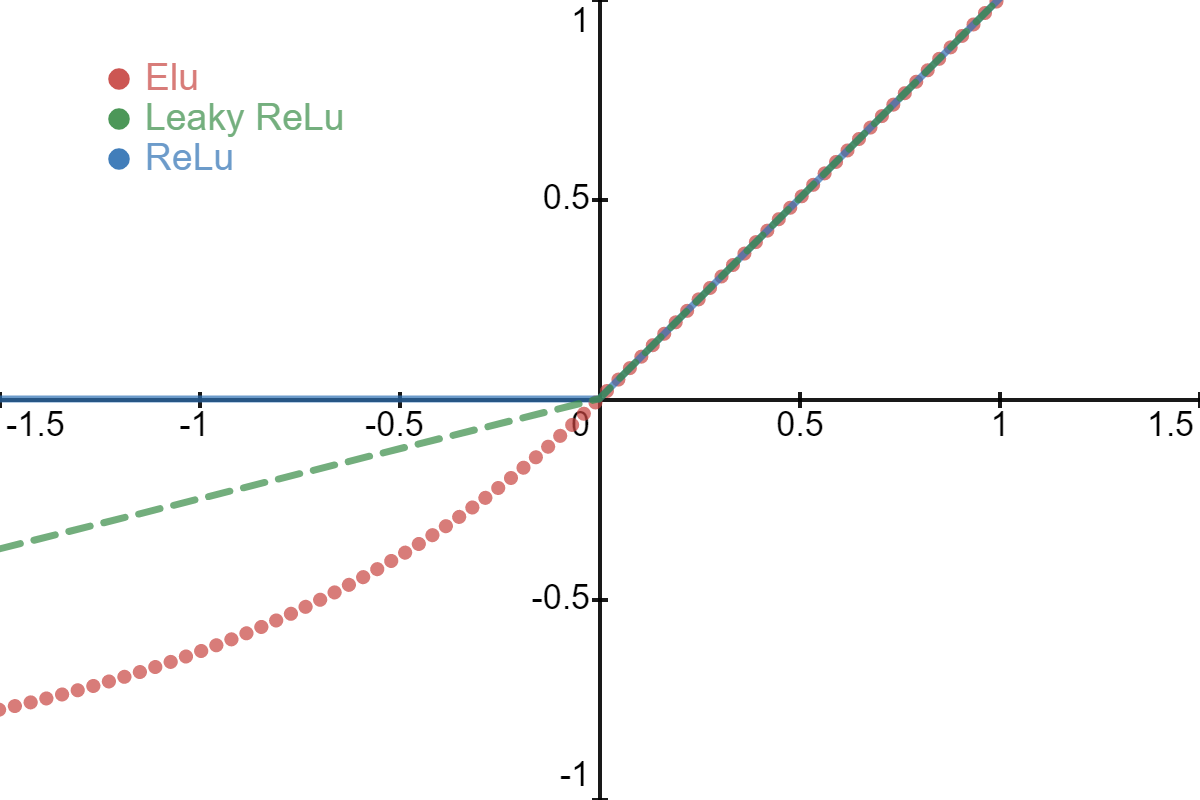
\includegraphics[width=.8\textwidth]{images/relu_elu-wide}
    \caption{Comparison of output of Elu, ReLu and Leaky ReLu activation functions on varying input values. If $x>0$, all activation functions have a linear output of $y=x$.}
    \label{fig:relu_elu}
\end{figure}
The second hyperparameter is the activation function of each neuron, the chosen activation function is applied on each layer, except for the final dense layer, which has a \textit{softmax} activation function (as explained in the \nameref{ch:method} chapter). I've included \textit{Rectified Linear Unit} (ReLu) \cite{Agarap2018deep} and \textit{Exponential Linear Unit} (Elu) as possible values. ReLu was included because it is seen as goto activation function, however because no negative activation is possible with this function, I've chosen to include Elu as activation function as well. Another alternative activation function close to ReLu allowing negative activation is Leaky ReLu, however this activation function was not available in Keras. A visualization of the different activation functions on varying input values can be found in \autoref{fig:relu_elu}.

\subsubsection{Pooling}
The output feature maps of convolutional layers are sensitive to the location of features in the input. One way of solving this problem is to down sample the feature maps. An approach to down sampling is provided in the form of a pooling layer. Two common types of pooling layers are defined: max and average. Max pooling works by returning the maximum value present in the pooling size as output, while average pooling works by calculating the average. The pooling layers defined in the models use local pooling with a pooling size of $2\times2$. 

Not only is pooling being used in convolutional networks, \textcite{Gimeno2020a} employ pooling between their bi-directional LSTM layers, that is why I have tested no pooling, max pooling and average pooling on both the CNN and LSTM models.

\subsubsection{Optimizer and Dropout}
Neural networks 'learn' by applying back propagation each learning iteration. During back propagation each weight is modified with regards to the output error. The aim is to reduce the value of the loss function. Because the models I created are multi-class classifiers with one true label, \textit{categorical cross entropy} is used as loss function in the models. Future research has to prove whether using other loss functions may be better instead \cite{Hsu2019multi}. To reduce the loss, the gradient is calculated. An optimizer is a function that can efficiently use this gradient to update the weights of the models to decrease the loss as fast as possible. One of the newest, most popular and best performing optimizers of this moment is the \textit{Adam} optimizer \cite{Kingma2014adam}. As comparison optimizer I've chosen the \textit{RMSprop} optimizer.

Another way of boosting the learning rate (or speed of which the loss decreases) is to use dropout. Dropout, introduced by \textcite{Hinton2012improving}, works by randomly 'dropping' a percentage of the neurons of certain layers. This means that all connections to these neurons are removed and that the other neurons are required to 'learn' the same representations that were first captured by the now removed neurons. Too low values for dropout are found to not have much impact, while too high dropout rates will reduce the overall performance of the models. 50\% dropout rate is generally seen as a the threshold from which the performance of the models will decrease, but still very much used \cite{Ullrich2014boundary}. I've therefore defined the set of dropout rates to range between 10\% and 50\% with a step size of 10\%. The dropout is applied on each layer except for the last dense layer.

\subsubsection{Epochs and Batch Size}
The final two parameters are used during the training phase of a model. These are the \textit{epochs} and \textit{batch size}. The amount of epochs defines how many times the training data is evaluated before the final model is returned. Increasing the amount of epochs means that the model has more time to learn all patterns into greater detail, however to high values will cause the model to overfit\footnote{If the model sees each sample many times it will become very good in classifying each sample, however new samples (less similar to the learned samples) will get a wrong classification more often.} and severely increases the time it takes to train the model. I've chosen to test models on 1, 10, 50 and 100 epochs (more epochs are being used in the field, this however would've made the training process all the much longer).

The batch size determines how many samples are passed through the network before back propagation is applied. The back propagation then is applied with the gradient of the loss of all these samples. Larger batch size generally speeds up the learning process of a model since less updates per epoch are performed. However, if the batch size is too large, a model will not always be able to learn specific patterns for one specific output, thus lowering its precision. I've chosen to create models with a wide range of batch size: 1, 5, 10, 50 and 100.

\subsubsection{Feature Combinations}
\begin{table}[t]
    \centering
    \begin{tabular}{|l|}
    \hline
    \textbf{Feature Combination}             \\ \hline\hline
    CQT, CENS, PCP, Tonnetz, MFCC, Tempogram \\ \hline
    CQT, MFCC                                \\ \hline
    CENS, MFCC                               \\ \hline
    PCP, MFCC                                \\ \hline
    Tonnetz, MFCC                            \\ \hline
    CQT, MFCC, Tempogram                     \\ \hline
    CENS, MFCC, Tempogram                    \\ \hline
    PCP, MFCC, Tempogram                     \\ \hline
    Tonnetz, MFCC, Tempogram                 \\ \hline
    CQT, Tempogram                           \\ \hline
    CENS, Tempogram                          \\ \hline
    PCP, Tempogram                           \\ \hline
    Tonnetz, Tempogram                       \\ \hline
    MFCC, Tempogram                          \\ \hline
    \end{tabular}
    \caption{Initial feature combinations.}
    \label{tab:init_feature_combo}
\end{table}
Based on previous research and type of each feature I've created 14 different sets of feature combinations, these can be found in \autoref{tab:init_feature_combo}. I've chosen to include a combination of all features extracted, combined with each feature paired with the MFCC, based on its overall high success rate in other research.

I've also included one a few of the possible chroma feature combined with one timbre feature combined with the tempogram combinations. To evaluate the performance of the tempogram I've included the pairing with each other feature to the feature combinations as well. The combinations missing are combinations of different timbre features and combinations of different chroma features, since combining a feature of one type with a feature of the same type will most likely not improve performance.

\subsubsection{Multi B-LSTM layer}
The LSTM models had one extra hyperparameter: whether to use a single or double B-LSTM layer. If a double LSTM layer model was made, and pooling was set to max or average, a pooling layer was put between the B-LSTM layers. Otherwise no pooling layer was used.


\section{Initial Test}
\subsection{Initial Test Setup}
 Using the possible values of each hyperparameter and the feature combinations an attempt had been made to create a model on each possible combination trained on 80\% of the total data (about 150000 samples) and evaluated on the remaining 20\% (35000). An output was registered of being correct when the index of neuron with the highest activation in the output layer corresponded with the index of the 1 in the one-hot-encoded true label vector and wrong otherwise. The accuracy was then calculated as the ratio of correct classifications to wrong classifications.

 One machine, containing an AMD Ryzen 7 3700x CPU and a NVIDIA GeForce GTX 1080 (8GB) GPU, was used to train and evaluate one CNN and one LSTM model simultaneously. Keras and the Tensorflow 2.0 backend were set to run on the GPU, while data flow was managed by the CPU.

\subsection{Initial Test Results}
Since both a CNN and LSTM model were trained simultaneously one epoch with a batch size of 1 roughly took $30\sim50$ seconds. A total of 50400 CNN models and 100800 LSTM models had to be trained. This means that about 6 million epochs of the data needed to be performed. Although only 20\% of the models have a batch size of 1, the expected time per epoch still was way above 10 seconds. This means that training and evaluating all CNN models would take 1 year and training all LSTM models around 2 years\footnote{Not counting the possible speedup when all CNN models have been evaluated. However, the very optimistic 10 seconds per epoch accounts for that.}.

Therefore the initial test setup was aborted after 1.5 weeks. In this time 145 LSTM and 292 CNN models were trained and evaluated. These models did not evaluate the impact of the amount of neurons, activation function and optimizer used nor the impact of the dropout. However, I was able to derive the impact of the amount of epochs, the batch size and feature combinations.

After preliminary data analysis, a number of trends were identified. The two trends that stood out the most were the amount of epochs and the batch size. A higher amount of epochs as well as a larger batch size always increased the performance of the model. The CQT turned out to be the best performing feature, with the Tempogram and MFCC being the two best features after that.   

The best performing CNN model had an accuracy of 0.66 on the test data, the best performing LSTM an accuracy of 0.43. No real performance increase of using a double B-LSTM layer over one B-LSTM layer was noticed.

\subsection{Adjustments}
To also be able to evaluate the other hyperparameter values, I made some changes to the search space.

\subsubsection{Feature Combinations}
\begin{table}[t]
    \centering
    \begin{tabular}{|l|}
    \hline
    \textbf{Feature Combination} \\ \hline\hline
    CQT, Tempogram               \\ \hline
    CQT, MFCC                    \\ \hline
    CQT, MFCC, Tempogram         \\ \hline
    \end{tabular}
    \caption{Final feature combinations.}
    \label{tab:final_feature_combo}
\end{table}
I first took a look at the feature combinations. The Tonnetz feature turned out to be too small of a feature to be usable with any pooling, and I therefore removed it from the features. Since no improvement was obtained using all features instead of only CQT, MFCC and Tempogram, the CENS and PCP features were removed from the feature combinations as well. This reduced the amount of feature combinations from 14 to 3. Thereby reducing the factor that determined the amount of models that had to be trained and evaluated the most. The final feature combinations can be found in \autoref{tab:final_feature_combo}.

\subsubsection{Hyperparameters}
After the feature combinations I've also reduced the amount of values of some hyperparameters. The most reduced ones are the epochs and batch size, these have been truncated to only contain 10, 50 and 100. Furthermore, I've reduced the dropout rates to 10\%, 25\% and 50\%. 

I've also trained the best performing CNN and LSTM on ReLu and Elu activation while using the Adam and RMSprop optimizer. This showed that using Elu did not improve the accuracy, while using the Adam optimizer heavily increased the accuracy with over 10\%. I therefore decided to use only ReLu as activation function and Adam optimizer as the only optimizer. As an additional benefit, Adam is a faster optimizer and therefore decreased the time of each epoch with quite a large factor. Furthermore, I removed the double B-LSTM layer hyperparameter, and chose to train only single B-LSTM layer models. The final hyperparameters and their values can be found in \autoref{tab:final_params}.

\subsubsection{Final Test}
\begin{table}[t]
    \centering
    \begin{tabular}{|l|l|}
    \hline
    \textbf{Hyperparameter} & \textbf{Values}                    \\ \hline\hline
    Neurons                 & 1285,256,512                       \\ \hline
    Activation function     & \textit{ReLu}                      \\ \hline
    Pooling                 & \textit{no\_pooling, max, average} \\ \hline
    Optimizer               & \textit{adam}                      \\ \hline
    Dropout                 & 10\%, 25\%, 50\%                   \\ \hline
    Epochs                  & 10, 50, 100                        \\ \hline
    Batch size              & 10, 50, 100                        \\ \hline
    \end{tabular}
    \caption{Final hyperparameters and their final range of values.}
    \label{tab:final_params}
\end{table}
One final big factor that increased the duration of each epoch was the amount of data. To decrease this heavy impacting factor, I've decided to take only 10\% of the original data as training and test data for the final test. The amount of samples used for training therefore decreased to 15000 and the amount of beats used for testing decreased to 3500. Although overall accuracy of the models were expected to be lower on this subset that on the full dataset, models with better hyperparameters and features will perform better than other models on both the full dataset or a subset thereof. Reducing the dataset too much can result in the training data not containing enough variation. I, however, expect 15000 samples to be quite representative for the full dataset, especially since all samples are chosen at random and not on a song basis. Each sample in this context means the concatenation of the feature vectors of the two beats before the current beat together with the feature vector of the current and the next beat.

The search space was now reduced to just above 700 different models. By using the Adam optimizer, removing the batch size of 1 and reducing the size of the dataset, the average time per epoch also reduced to around 3 seconds. The expected time to train and evaluate these models therefore reduced to less than a week, which was a lot more within the time-scope of this thesis. 


\section{Final Results}
% \begin{table}[t]
%     \centering
%     \begin{tabular}{|l|l|l|l|l|l|l|l|l|l|l|l|l|l|l|l|l|l|l|}
%     \hline
%                                                                                            & \multicolumn{3}{l|}{\textbf{Neuron Count}} & \multicolumn{3}{l|}{\textbf{Dropout}} & \multicolumn{3}{l|}{\textbf{Pooling}} & \multicolumn{3}{l|}{\textbf{Epochs}} & \multicolumn{3}{l|}{\textbf{Batch size}} & \multicolumn{3}{l|}{\textbf{Feature Combo}}                                                                                                                                         \\ \hline
%     \textbf{Values}                                                                        & 128          & 256          & 512          & 10\%        & 25\%       & 50\%       & none      & max        & average      & 10        & 50          & 100        & 10           & 50          & 100         & \begin{tabular}[c]{@{}l@{}}CQT +\\ Tempogram\end{tabular} & \begin{tabular}[c]{@{}l@{}}CQT +\\ MFCC\end{tabular} & \begin{tabular}[c]{@{}l@{}}CQT + MFCC +\\ Tempogram\end{tabular} \\ \hline
%     \textbf{\begin{tabular}[c]{@{}l@{}}Amount of models\\ created with value\end{tabular}} & 267          & 250          & 218          & 316         & 232        & 187        & 242       & 259        & 234          & 255       & 244         & 236        & 249          & 245         & 241         & 202                                                       & 201                                                  & 200                                                              \\ \hline
%     \textbf{\begin{tabular}[c]{@{}l@{}}Amount of models \\ in top 10\%\end{tabular}}       & 37           & 18           & 15           & 27          & 28         & 15         & 0         & 43         & 27           & 0         & 20          & 50         & 2            & 27          & 41          & 37                                                        & 0                                                    & 18                                                               \\ \hline
%     \textbf{\begin{tabular}[c]{@{}l@{}}Percentage of models\\ in top 10\%\end{tabular}}    & 0.139        & 0.072        & 0.069        & 0.085       & 0.121      & 0.080      & 0         & 0.166      & 0.115        & 0         & 0.082       & 0.212      & 0.008        & 0.110       & 0.170       & 0.183                                                     & 0                                                    & 0.090                                                            \\ \hline
%     \end{tabular}
%     \caption{Analysis of all models created with different parameter values and feature combinations}
%     \label{tab:model_analysis}
% \end{table}


% \begin{table}[t]
%     \centering
%     \begin{tabular}{|l||l|l|l|l|}
%     \hline
%                                             & \textbf{Values}                                                  & \textbf{\begin{tabular}[c]{@{}l@{}}No. models\\ created with value\end{tabular}} & \textbf{\begin{tabular}[c]{@{}l@{}}No. models\\in top 10\%\end{tabular}} & \textbf{\begin{tabular}[c]{@{}l@{}}\%. models\\in top 10\%\end{tabular}} \\ \hline\hline
%     \multirow{3}{*}{\textbf{Neuron\\Count}}  & 128                                                              & 267                                                                                    & 37                                                                               & \textbf{0.139}                                                                      \\ \cline{2-5} 
%                                             & 256                                                              & 250                                                                                    & 18                                                                               & 0.072                                                                               \\ \cline{2-5} 
%                                             & 512                                                              & 218                                                                                    & 15                                                                               & 0.069                                                                               \\ \hline
%     \multirow{3}{*}{\textbf{Dropout}}       & 10\%                                                             & 316                                                                                    & 27                                                                               & 0.085                                                                               \\ \cline{2-5} 
%                                             & 25\%                                                             & 232                                                                                    & 28                                                                               & \textbf{0.121}                                                                      \\ \cline{2-5} 
%                                             & 50\%                                                             & 187                                                                                    & 15                                                                               & 0.080                                                                               \\ \hline
%     \multirow{3}{*}{\textbf{Pooling}}       & none                                                             & 242                                                                                    & 0                                                                                & 0                                                                                   \\ \cline{2-5} 
%                                             & max                                                              & 259                                                                                    & 43                                                                               & \textbf{0.166}                                                                      \\ \cline{2-5} 
%                                             & average                                                          & 234                                                                                    & 27                                                                               & 0.115                                                                               \\ \hline
%     \multirow{3}{*}{\textbf{Epochs}}        & 10                                                               & 255                                                                                    & 0                                                                                & 0                                                                                   \\ \cline{2-5} 
%                                             & 50                                                               & 244                                                                                    & 20                                                                               & 0.082                                                                               \\ \cline{2-5} 
%                                             & 100                                                              & 236                                                                                    & 50                                                                               & \textbf{0.212}                                                                      \\ \hline
%     \multirow{3}{*}{\textbf{Batch\\size}}    & 10                                                               & 249                                                                                    & 2                                                                                & 0.008                                                                               \\ \cline{2-5} 
%                                             & 50                                                               & 245                                                                                    & 27                                                                               & 0.110                                                                               \\ \cline{2-5} 
%                                             & 100                                                              & 241                                                                                    & 41                                                                               & \textbf{0.170}                                                                      \\ \hline
%     \multirow{3}{*}{\textbf{Feature\\Combo}} & \begin{tabular}[c]{@{}l@{}}CQT +\\ Tempogram\end{tabular}        & 202                                                                                    & 37                                                                               & \textbf{0.183}                                                                      \\ \cline{2-5} 
%                                             & \begin{tabular}[c]{@{}l@{}}CQT +\\ MFCC\end{tabular}             & 201                                                                                    & 0                                                                                & 0                                                                                   \\ \cline{2-5} 
%                                             & \begin{tabular}[c]{@{}l@{}}CQT + MFCC +\\ Tempogram\end{tabular} & 200                                                                                    & 18                                                                               & 0.090                                                                               \\ \hline
%     \end{tabular}
% \end{table}

% Please add the following required packages to your document preamble:
% \usepackage{multirow}
\begin{table}[t]
    \centering
    \begin{tabular}{|l||l|l|l|l|}
    \hline
                                                                                       & \textbf{Values}                                                  & \textbf{\begin{tabular}[c]{@{}l@{}}No. models\\ created\end{tabular}} & \textbf{\begin{tabular}[c]{@{}l@{}}No. models \\ in top 10\%\end{tabular}} & \textbf{\begin{tabular}[c]{@{}l@{}}\%. models\\ in top 10\%\end{tabular}} \\ \hline\hline
    \multirow{3}{*}{\textbf{\begin{tabular}[c]{@{}l@{}}Neuron \\ Count\end{tabular}}}  & 128                                                              & 267                                                                   & 37                                                                         & \textbf{0.139}                                                            \\ \cline{2-5} 
                                                                                       & 256                                                              & 250                                                                   & 18                                                                         & 0.072                                                                     \\ \cline{2-5} 
                                                                                       & 512                                                              & 218                                                                   & 15                                                                         & 0.069                                                                     \\ \hline\hline
    \multirow{3}{*}{\textbf{Dropout}}                                                  & 10\%                                                             & 316                                                                   & 27                                                                         & 0.085                                                                     \\ \cline{2-5} 
                                                                                       & 25\%                                                             & 232                                                                   & 28                                                                         & \textbf{0.121}                                                            \\ \cline{2-5} 
                                                                                       & 50\%                                                             & 187                                                                   & 15                                                                         & 0.080                                                                     \\ \hline\hline
    \multirow{3}{*}{\textbf{Pooling}}                                                  & none                                                             & 242                                                                   & 0                                                                          & 0                                                                         \\ \cline{2-5} 
                                                                                       & max                                                              & 259                                                                   & 43                                                                         & \textbf{0.166}                                                            \\ \cline{2-5} 
                                                                                       & average                                                          & 234                                                                   & 27                                                                         & 0.115                                                                     \\ \hline\hline
    \multirow{3}{*}{\textbf{Epochs}}                                                   & 10                                                               & 255                                                                   & 0                                                                          & 0                                                                         \\ \cline{2-5} 
                                                                                       & 50                                                               & 244                                                                   & 20                                                                         & 0.082                                                                     \\ \cline{2-5} 
                                                                                       & 100                                                              & 236                                                                   & 50                                                                         & \textbf{0.212}                                                            \\ \hline\hline
    \multirow{3}{*}{\textbf{\begin{tabular}[c]{@{}l@{}}Batch \\ size\end{tabular}}}    & 10                                                               & 249                                                                   & 2                                                                          & 0.008                                                                     \\ \cline{2-5} 
                                                                                       & 50                                                               & 245                                                                   & 27                                                                         & 0.110                                                                     \\ \cline{2-5} 
                                                                                       & 100                                                              & 241                                                                   & 41                                                                         & \textbf{0.170}                                                            \\ \hline\hline
    \multirow{3}{*}{\textbf{\begin{tabular}[c]{@{}l@{}}Feature \\ Combo\end{tabular}}} & \begin{tabular}[c]{@{}l@{}}CQT +\\ Tempogram\end{tabular}        & 202                                                                   & 37                                                                         & \textbf{0.183}                                                            \\ \cline{2-5} 
                                                                                       & \begin{tabular}[c]{@{}l@{}}CQT +\\ MFCC\end{tabular}             & 201                                                                   & 0                                                                          & 0                                                                         \\ \cline{2-5} 
                                                                                       & \begin{tabular}[c]{@{}l@{}}CQT + MFCC +\\ Tempogram\end{tabular} & 200                                                                   & 18                                                                         & 0.090                                                                     \\ \hline
    \end{tabular}
    \caption{Analysis of all CNN models created with different parameter values and feature combinations. Best performing value of each parameter had been put in bold.}
    \label{tab:model_analysis}
\end{table}
After 5 days all models were trained and evaluated. The accuracy of each model was saved in a text file, named by the parameter values and features used to create that model separated by an underscore. All models were then grouped in a list sorted by their accuracy in descending order. I analysed each parameter by grouping all models by their value for that parameter. Then I counted the total amount of models made with that value for the parameter and amount of models in the top 10\% of all models (around 700 models were created, top 10\% therefore accounted for 70 models). With these counts I calculated the percentage of models with that value in the top 10\% of models. This gives a distribution of best performing parameter value on the top 30\% of all models. All distributions can be found in \autoref{tab:model_analysis}.

Using the percentages, a best performing value for each parameter can be derived. This does not immediately mean that the best performing models has these values for each parameter, however further analysis showed that the model with these parameter values and feature combination as input, indeed was among the top 3 best performing models. 

\subsection{Best performing CNN and LSTM models}
\subsubsection{Parameter values and input features combination}
Following the analysis of the parameter values, I've defined the best performing CNN and LSTM models. These models both have a neuron count of 128 in the first layer, a dropout of 25\%, max pooling, a batch size and epoch count of 100, ReLu activation function and Adam optimizer. As input features I've chosen the Constant-Q Transform in combination with the Tempogram. Using the best performing values for each parameter together with all features as input only improved the accuracy with $<1$\%, while increasing evaluation time. The LSTM model has only one B-LSTM layer, since adding more layers did not improve its accuracy but instead added more time to the training and evaluation time of the model.

\subsubsection{Evaluation of best models on different datasets}
% \begin{table}[t]    
%     \begin{tabular}{lll}
%                       & CNN    & LSTM   \\
%     Training Accuracy & 0.9456 & 0.8265 \\
%     Test Accuracy     & 0.80   & 0.77   \\
%     1200 Accuracy     & 0.89   & 0.84  
%     \end{tabular}
%     \label{tab:final_results}
% \end{table}

%%%%%%%%%%%%%%%%%%
% Too wide table %
%%%%%%%%%%%%%%%%%%
% \begin{table}[t]
%     \centering
%     \begin{tabular}{|l|l|l|l|l|l|l|l|l|l|l|l|}
%     \hline
%     \multirow{2}{*}{}              & \multicolumn{2}{l|}{\textbf{Beat Classification Accuracy}} & \multirow{2}{*}{} & \multicolumn{2}{l|}{\textbf{\begin{tabular}[c]{@{}l@{}}All songs own\\ ground truth\end{tabular}}} & \multicolumn{2}{l|}{\textbf{\begin{tabular}[c]{@{}l@{}}All songs SALAMI\\ ground truth\end{tabular}}} & \multicolumn{2}{l|}{\textbf{\begin{tabular}[c]{@{}l@{}}SALAMI song-id 1200 own\\ ground truth\end{tabular}}} & \multicolumn{2}{l|}{\textbf{\begin{tabular}[c]{@{}l@{}}SALAMI song-id 1200 SALAMI\\ ground truth\end{tabular}}} \\ \cline{2-3} \cline{5-12} 
%                                    & Training data                 & Test data                  &                   & Non-Trimmed                                        & Trimmed                                       & Non-Trimmed                                         & Trimmed                                         & Non-Trimmed                                             & Trimmed                                            & Non-Trimmed                                              & Trimmed                                              \\ \hline
%     \multirow{2}{*}{\textbf{CNN}}  & \multirow{2}{*}{0.9456}       & \multirow{2}{*}{0.80}      & 0.5F              & 0.6849                                             & 0.5627                                        & 0.1451                                              & 0.0374                                          & 0.6087                                                  & 0.5261                                             & 0.55                                                     & 0.48                                                 \\ \cline{4-12} 
%                                    &                               &                            & 3F                & 0.8545                                             & 0.7935                                        & 0.3397                                              & 0.1960                                          & 0.9565                                                  & 0.9474                                             & 0.69                                                     & 0.64                                                 \\ \hline
%     \multirow{2}{*}{\textbf{LSTM}} & \multirow{2}{*}{0.8265}       & \multirow{2}{*}{0.77}      & 0.5F              & 0.4526                                             & 0.3003                                        & 0.1474                                              & 0.0581                                          & 0.3846                                                  & 0.2727                                             & 0.38                                                     & 0.29                                                 \\ \cline{4-12} 
%                                    &                               &                            & 3F                & 0.6141                                             & 0.5065                                        & 0.3487                                              & 0.2296                                          & 0.6923                                                  & 0.6364                                             & 0.56                                                     & 0.50                                                 \\ \hline
%     \end{tabular}
%     \caption{Final Results}
%     \label{tab:final_results}
% \end{table}

% Please add the following required packages to your document preamble:
% \usepackage{multirow}
\begin{table}[t]
    \centering
    \begin{tabular}{|l|l||l|l|l|l|}
    \hline
                                                                                             \textbf{Dataset} & \textbf{Measure} & \multicolumn{2}{l|}{\textbf{CNN}} & \multicolumn{2}{l|}{\textbf{LSTM}} \\ \hline\hline
    \multirow{2}{*}{\textbf{\begin{tabular}[c]{@{}l@{}}Beat Classification \\ Accuracy\end{tabular}}}            & Training data & \multicolumn{2}{l|}{0.9456}       & \multicolumn{2}{l|}{0.8265}        \\ \cline{2-6} 
                                                                                                                 & Test data     & \multicolumn{2}{l|}{0.80}         & \multicolumn{2}{l|}{0.77}          \\ \hline\hline
    \multicolumn{2}{|l|}{}                                                                                                       & \textbf{0.5F}   & \textbf{3F}     & \textbf{0.5F}    & \textbf{3F}     \\ \hline
    \multirow{2}{*}{\textbf{\begin{tabular}[c]{@{}l@{}}All songs \\ own ground truth\end{tabular}}}              & Untrimmed   & 0.6849          & 0.8545          & 0.4526           & 0.6141          \\ \cline{2-6} 
                                                                                                                 & Trimmed       & 0.5627          & 0.7935          & 0.3003           & 0.5065          \\ \hline
    \multirow{2}{*}{\textbf{\begin{tabular}[c]{@{}l@{}}All songs \\ SALAMI ground truth\end{tabular}}}           & Untrimmed   & 0.1451          & 0.3397          & 0.1474           & 0.3487          \\ \cline{2-6} 
                                                                                                                 & Trimmed       & 0.0374          & 0.1960          & 0.0581           & 0.2296          \\ \hline
    \multirow{2}{*}{\textbf{\begin{tabular}[c]{@{}l@{}}SALAMI song-id 1200 \\ own ground truth\end{tabular}}}    & Untrimmed   & 0.6087          & 0.9565          & 0.3846           & 0.6923          \\ \cline{2-6} 
                                                                                                                 & Trimmed       & 0.5261          & 0.9474          & 0.2727           & 0.6364          \\ \hline
    \multirow{2}{*}{\textbf{\begin{tabular}[c]{@{}l@{}}SALAMI song-id 1200 \\ SALAMI ground truth\end{tabular}}} & Untrimmed   & 0.55            & 0.69            & 0.38             & 0.56            \\ \cline{2-6} 
                                                                                                                 & Trimmed       & 0.48            & 0.64            & 0.29             & 0.50            \\ \hline
    \end{tabular}
    \caption{An overview of the final CNN and LSTM model evaluated on multiple datasets. The training- and testset accuracy is evaluated using Keras. The F-measures on SALAMI 1200 (custom and original ground truth) as well as the F-measures on the full SALAMI dataset (custom and original ground truth) are calculated using the MSAF. In all cases the same CNN or LSTM model were used, these are the ones trained on the custom ground truth (9 unique output labels).} 
    \label{tab:final_results}
\end{table}
I then trained each best model on the full dataset, with 80\% of the dataset as training data and the remaining 20\% as test data. The accuracy on the training and test data were 94.56\% and 80\% for the CNN model and 82.65\% and 77\% for the LSTM model respectively (\autoref{tab:final_results} first row). These models were then saved in \textit{.h5} file. This file format is used by Keras to models with their trained weights. This way inference can be easily applied on another machine, since the model only needs to be loaded instead of fully trained\footnote{It can also be used to further train the network on other or more data on another machine and than re-saved as \textit{.h5} file, however this is less common in practice.}.

Since the end goal was to segment a song into \textit{chorus}, \textit{verse}, etc. instead of predicting a single beat, I've taken a few arbitrary songs from the dataset. Then I looked at the amount of segments and the amount of different labels. Based on this I've taken SALAMI song-id 1200 as my test song for the final models. To perform the test I've sequentially inferred the label of each beat of the song with each model. As expected there were some beats that had another label than the labels of a number of beats around it. This is due to the less than 100\% accuracy of the models on the dataset (which is to be desired, since they would be overfitted otherwise). 

\subsubsection{Label Filtering Function}
\begin{table}[t]
    \centering
    \begin{tabular}{|l|l|l|l|l|}
    \hline
    \textbf{Beat} & \textbf{Beat Start Time} & \textbf{True Label} & \textbf{Predicted Label} & \textbf{Filtered Label} \\ \hline\hline
    0             & 1.253877551020408  & no\_function        & no\_function             & no\_function            \\ \hline
    1             & 1.764716553287982  & no\_function        & no\_function             & no\_function            \\ \hline
    2             & 2.321995464852609  & no\_function        & no\_function             & no\_function            \\ \hline
    3             & 2.832834467120181  & no\_function        & no\_function             & no\_function            \\ \hline
    4             & 3.390113378684807  & no\_function        & no\_function             & no\_function            \\ \hline
    5             & 3.900952380952381  & intro               & intro                    & intro                   \\ \hline
    6             & 4.458231292517007  & intro               & intro                    & intro                   \\ \hline
    7             & 4.96907029478458   & intro               & intro                    & intro                   \\ \hline
    8             & 5.479909297052155  & intro               & intro                    & intro                   \\ \hline
    9             & 6.03718820861678   & intro               & intro                    & intro                   \\ \hline
    10            & 6.548027210884354  & intro               & intro                    & intro                   \\ \hline
    11            & 7.058866213151927  & intro               & intro                    & intro                   \\ \hline
    12            & 7.569705215419501  & intro               & verse                    & intro                   \\ \hline
    13            & 8.080544217687075  & intro               & intro                    & intro                   \\ \hline
    14            & 8.591383219954649  & intro               & solo                     & intro                   \\ \hline
    15            & 9.102222222222222  & intro               & intro                    & intro                   \\ \hline
    \dots         & \dots              & \dots               & \dots                    & \dots                   \\ \hline
    \dots         & \dots              & \dots               & \dots                    & \dots                   \\ \hline
    \dots         & \dots              & \dots               & \dots                    & \dots                   \\ \hline
    453           & 238.3760544217687  & solo                & solo                     & solo                    \\ \hline
    454           & 238.8868934240363  & solo                & solo                     & solo                    \\ \hline
    455           & 239.3977324263039  & solo                & no\_function             & solo                    \\ \hline
    456           & 239.9085714285714  & solo                & solo                     & solo                    \\ \hline
    457           & 240.419410430839   & solo                & solo                     & solo                    \\ \hline
    458           & 240.9302494331066  & solo                & solo                     & solo                    \\ \hline
    459           & 241.4410884353742  & solo                & solo                     & solo                    \\ \hline
    460           & 241.9519274376417  & solo                & solo                     & solo                    \\ \hline
    461           & 242.4627664399093  & solo                & solo                     & solo                    \\ \hline
    462           & 242.9271655328798  & solo                & chorus                   & solo                    \\ \hline
    463           & 243.3915646258504  & solo                & chorus                   & solo                    \\ \hline
    464           & 243.8559637188209  & solo                & solo                     & solo                    \\ \hline
    465           & 244.3668027210885  & solo                & solo                     & solo                    \\ \hline
    466           & 244.8776417233560  & solo                & solo                     & solo                    \\ \hline
    467           & 245.3884807256236  & solo                & solo                     & solo                    \\ \hline
    468           & 245.8528798185941  & solo                & no\_function             & solo                    \\ \hline
    \end{tabular}
    \caption{First and last 50 beats of SALAMI 1200 true, predicted and filtered labels produced by best CNN model.}
    \label{tab:1200_cnn}
\end{table}
\begin{table}[t]
    \centering
    \begin{tabular}{|l|l|l|l|l|}
    \hline
    \textbf{Beat}        & \textbf{Beat Start Time}   & \textbf{True Label}  & \textbf{Predicted Label} & \textbf{Filtered Label} \\ \hline\hline
    0                    & 1.25387755102041     & no\_function         & no\_function             & no\_function            \\ \hline
    1                    & 1.764716553287982    & no\_function         & no\_function             & no\_function            \\ \hline
    2                    & 2.321995464852608    & no\_function         & no\_function             & no\_function            \\ \hline
    3                    & 2.832834467120181    & no\_function         & no\_function             & no\_function            \\ \hline
    4                    & 3.390113378684807    & no\_function         & no\_function             & no\_function            \\ \hline
    5                    & 3.900952380952381    & intro                & no\_function             & no\_function            \\ \hline
    6                    & 4.458231292517007    & intro                & intro                    & intro                   \\ \hline
    7                    & 4.96907029478458     & intro                & intro                    & intro                   \\ \hline
    8                    & 5.479909297052155    & intro                & intro                    & intro                   \\ \hline
    9                    & 6.03718820861678     & intro                & intro                    & intro                   \\ \hline
    10                   & 6.548027210884354    & intro                & intro                    & intro                   \\ \hline
    11                   & 7.058866213151927    & intro                & intro                    & intro                   \\ \hline
    12                   & 7.569705215419501    & intro                & intro                    & intro                   \\ \hline
    13                   & 8.080544217687075    & intro                & intro                    & intro                   \\ \hline
    14                   & 8.591383219954649    & intro                & intro                    & intro                   \\ \hline
    15                   & 9.102222222222222    & intro                & intro                    & intro                   \\ \hline
    \dots                & \dots                & \dots                & \dots                    & \dots                   \\ \hline
    \dots                & \dots                & \dots                & \dots                    & \dots                   \\ \hline
    \dots                & \dots                & \dots                & \dots                    & \dots                   \\ \hline
    453                  & 238.3760544217687    & solo                 & solo                     & solo                    \\ \hline
    454                  & 238.8868934240363    & solo                 & solo                     & solo                    \\ \hline
    455                  & 239.3977324263039    & solo                 & solo                     & solo                    \\ \hline
    456                  & 239.9085714285714    & solo                 & solo                     & solo                    \\ \hline
    457                  & 240.419410430839     & solo                 & solo                     & solo                    \\ \hline
    458                  & 240.9302494331066    & solo                 & solo                     & solo                    \\ \hline
    459                  & 241.4410884353742    & solo                 & solo                     & solo                    \\ \hline
    460                  & 241.9519274376417    & solo                 & chorus                   & solo                    \\ \hline
    461                  & 242.4627664399093    & solo                 & solo                     & solo                    \\ \hline
    462                  & 242.9271655328798    & solo                 & solo                     & solo                    \\ \hline
    463                  & 243.3915646258504    & solo                 & solo                     & solo                    \\ \hline
    464                  & 243.8559637188209    & solo                 & solo                     & solo                    \\ \hline
    465                  & 244.3668027210885    & solo                 & solo                     & solo                    \\ \hline
    466                  & 244.8776417233560    & solo                 & verse                    & solo                    \\ \hline
    467                  & 245.3884807256236    & solo                 & solo                     & solo                    \\ \hline
    468                  & 245.8528798185941    & solo                 & chorus                   & solo                    \\ \hline
    \end{tabular}
    \caption{First and last 15 beats of SALAMI 1200 true, predicted and filtered labels produced by best LSTM model.}
    \label{tab:1200_lstm}
\end{table}
To still be able to use the start of a sequence of new labels as start of a segment I wrote a simple filtering function, based on the predictions on SALAMI 1200. This functions works by iterating over all the predicted labels of the beats. When a label different to the label of the beat before it is detected, the next 4 beats are scanned. If the label of the previous beat is detected in the labels of the next 4 beats, that label is taken as filtered label, otherwise the predicted label is taken as filtered label. This function thus requires each segment to be at least 5 beats in length, which is quite common in the ground truth I created based on the label grouping mentioned in \nameref{sec:3.the_data} section in \autoref{ch:method}. In the SALAMI dataset this is less common, but I will elaborate on this in the \nameref{ch:discussion} chapter.

I have also tried another filtering function. This function worked similar to the filtering function I used, however instead of checking if the label of the previous beat occurs in the labels of the next 4 beats, the most occurring label of the next 5 beats was taken as filtered label. The problem of this function was that if there were 3 falsely classified beats among the next 5 beats, this was taken as filtered label, thus causing a short, falsely classified segment to occur in the filtered predictions. This function also required segments of at least 6 beats, 1 beat (about 0.5 seconds) longer than the other filtering function, which can already be quite impactful.\\

The ground truth, predicted and filtered output of the CNN model on the first and last 15 beats of SALAMI 1200 can be found in \autoref{tab:1200_cnn}, the same output of the LSTM model on the first and last 15 beats of SALAMI 1200 can be found in \autoref{tab:1200_lstm}.

\subsubsection{Final Evaluation on SALAMI and own Ground Truth}
Using the filtering function I described earlier, I was able to create a \textit{JSON Annotated Music Specification} (JAMS) file \cite{Humphrey2014jams} of each song from the dataset. I also created a JAMS file for each ground truth I created. I then used the Music Structure Analysis Framework (MSAF) \cite{Nieto2016systematic} to evaluate the filtered segments of the CNN and LSTM models on both the SALAMI and my own ground truths.

The MSAF returns quite an extensive evaluation report. To enhance overview, I have only included the (mean) F-measures from the reports. Four different F-measures are returned with each report. An F-measure of an evaluation of the segment boundary location with a 0.5 second and 3 seconds time tolerance to the ground truth, both trimmed and untrimmed. MSAF automatically adds a segment boundary at the start and end of a song, if the untrimmed F-measure is calculated, these segment boundaries are included in the calculation. If a trimmed F-measure is calculated, these segment boundaries are excluded from the calculation, often lowering the F-measure, since only the segment boundaries produced by the models are now taken into account.

All F-measures can be found in \autoref{tab:final_results}, the full ground truth, predicted and filtered labels of SALAMI 1200 of the CNN \href{https://git.science.uu.nl/l.m.vanboven/bachelor-scriptie-musical-sctructure-analysis/-/blob/master/Leander/Results_Analysis/1200_cnn.csv}{here (link)}, and the same data of the LSTM \href{https://git.science.uu.nl/l.m.vanboven/bachelor-scriptie-musical-sctructure-analysis/-/blob/master/Leander/Results_Analysis/1200_lstm.csv}{here (link)}.